\documentclass[a4paper,12pt]{ctexbook}
\usepackage[margin=1cm]{geometry}
\usepackage{graphicx}
\usepackage{subfigure}
\usepackage{float}
\usepackage[colorlinks,linkcolor=black]{hyperref}%colorlinks启用链接颜色,linkcolor指定对应的颜色
\usepackage{listings}
%\usepackage[cache=false]{minted}  % 代码高亮X
\usepackage{fontspec}
\usepackage{tikz,xcolor,mwe}

\definecolor{cvgreen}{HTML}{92D14F}
\definecolor{cvgray}{HTML}{D8E4BE}
\definecolor{cvtext}{HTML}{92909B}
\usetikzlibrary{shadows}

\pagestyle{empty}
\CTEXsetup[format={\large\bfseries}]{section}%可以让section的标题左对齐。
\CTEXsetup[format={\Large\bfseries}]{chapter}%可以让chapter的标题左对齐。
%\CTEXsetup[format+={\flushleft}]{section}%让section的标题居左
%\renewcommand{\thesection}{\chinese{section}}%将“1.1”改为汉字“一”,但是subsection就会变成  六.1 ,比较难看,还是不用比较好。

\begin{document}


\begin{tikzpicture}[remember picture,overlay]
\fill[cvgreen] (current page.north west) rectangle ([xshift=6cm]current page.south west);% green bar
\fill[cvgray] ([yshift=-11cm]current page.north west) rectangle ([yshift=-17cm]current page.north east); % gray bar

\node[cvtext,right] at ([xshift=3.5cm,yshift=-13cm]current page.north west) {\Huge Machine Learning way};
\node[cvtext,above left] at ([xshift=-1cm,yshift=-16.5cm]current page.north east) {\Large\bfseries \today};
% cover photo
\node[inner sep=0pt,below right] (image) at ([xshift=17cm,yshift=-1cm]current page.north west) {
\includegraphics[width=3cm]{hainulogo.png}};
% name and address
\node[fill=white,align=center,text width=6.4cm,inner sep=0.8cm,below] (name) at (image.south) {};
\node[text width=15cm,inner sep=0.3cm,below right] at (name.south west){\Large Author:Flynn\\E-Mail:zofon@qq.com};
% attachments
\node[white,text width=5cm,inner sep=0.6cm,above right] at ([yshift=1cm]current page.south west)
{\large\obeylines\textbf{This is\\Open Source}};
\end{tikzpicture}

\tableofcontents

\chapter{相关的概念}
在学习机器学习之前首先要了解一些相关的概念。\cite{Johnson2015}
\begin{description}
  \item[AI] 人工智能是最早出现的,也是最大、最外侧的同心圆;\cite{深度学习框架的评估与比较_孙镜涛}
  \item[ML] 机器学习
  \item[DL] 深度学习,深度学习造成了前所未有的巨大的影响, 是当今人工智能大爆炸的核心驱动。
\end{description}
五十年代,人工智能曾一度被极为看好。之后,人工智能的一些较小的子集发展了起来。先是机器学习,然后是深度学习。深度学习又是机器学习的子集。。

早在1956年夏天那次会议,人工智能的先驱们就梦想着用当时刚刚出现的计算机来构造复杂的、拥有与人类智慧同样本质特性的机器。这就是我们现在所说的“强人工智能”(General AI)。这个无所不能的机器,它有着我们所有的感知(甚至比人更多),我们所有的理性,可以像我们一样思考。

人们在电影里也总是看到这样的机器:友好的,像星球大战中的C-3PO;邪恶的,如终结者。强人工智能现在还只存在于电影和科幻小说中,原因不难理解,我们还没法实现它们,至少目前还不行。

我们目前能实现的,一般被称为“弱人工智能”(Narrow AI)。弱人工智能是能够与人一样,甚至比人更好地执行特定任务的技术。例如,Pinterest上的图像分类;或者Facebook的人脸识别。

这些是弱人工智能在实践中的例子。这些技术实现的是人类智能的一些具体的局部。但它们是如何实现的?这种智能是从何而来?这就带我们来到同心圆的里面一层,机器学习。

%
\chapter{如何研究学习一个机器学习算法}
中文:\url{http://blog.jobbole.com/80658/}
英文:\url{http://machinelearningmastery.com/how-to-investigate-machine-learning-algorithm-behavior/}
\section{引言}
机器学习算法都是一个个复杂的体系,需要通过研究来理解。学习算法的静态描述是一个好的开始,但是这并不足以使我们理解算法的行为,我们需要在动态中来理解算法。

机器学习算法的运行实验,会使你对于不同类型问题得出的实验结论,并对实验结论与算法参数两者的因果关系有一个直观认识。

在这篇文章中,你将会知道怎么研究学习一个机器学习算法。你将会学到5个简单步骤,你可以用来设计和完成你的第一个机器学习算法实验

你会发现机器学习实验不光是学者们的专利,你也可以;你也会知道实验是通往精通的必经之路,因为你可以从经验中学到因果关系的知识, 这是其它地方学不到的。

\section{什么是研究机器学习算法}
当研究一个机器学习算法的时候,你的目标是找到可得到好结果的机器算法行为,这些结果是可以推广到多个问题或者多个类型的问题上。

你通过对算法状态做系统研究来研究学习机器学习算法。这项工作通过设计和运行可控实验来完成

一旦你完成了一项实验,你可以对结论作出解释和提交。这些结论会让你得以管窥在算法变化中因果关系。这就是算法行为和你获得的结论间的关系。

\section{怎样研究学习机器学习算法}
在这一部分,我们将学到5个简单的步骤,你可以通过它来研究学习一个机器算法
\subsection{选择一个算法}
选择一个你有疑问的算法

这个算法可能是你正在某个问题上应用的,或者你发现在其他环境中表现很好,将来你想使用

就实验的意图来说,使用现成的算法是有帮助的。这会给你一个底线:存在bug几率最低

自己实现一个算法可能是了解算法过程的一个好的方式,但是,实验期间,会引入额外的变量,比如bug,和大量必须为算法所做的微观决策
\subsection{确定一个问题}
你必须有一个你试图寻找答案的研究问题。问题越明确,问题越有用

给出的示例问题包括以下几个方面:

KNN算法中,作为样本空间中的一部分的K值在增大时有什么影响?

在SVM算法中,选择不同的核函数在二分类问题上有什么影响 ?

在二分类问题中,逻辑回归上的不同参数的缩放有什么影响 ?

在随机森林模型中,在训练集上增加任意属性对在分类准确性上有什么影响?

针对算法,设计你想回答的问题。仔细考虑,然后列出5个逐渐演变的问题,并且深入推敲那个最精确的
\subsection{设计实验}
从你的问题中挑选出关键元素然后组成你的实验内容。 例如,拿上面的示例问题为例:“二元分类问题中逻辑回归上的不同的参数缩放有什么影响?”

你从这个问题中挑出来用来设计实验的元素是:

属性缩放法:你可以采用像正态化、标准化,将某一属性提升至乘方、取对数等方法

逻辑回归:你想使用哪种已经实现的逻辑回归。

二元分类问题:存在数值属性不同的二分类问题标准。需要准备多种问题,其中一些问题的规模是相同的(像电离层),然而其他一些问题的属性有不同的缩放值(像糖尿病问题)。

性能: 类似分类准确性的模型性能分数是需要的

花时间仔细挑选你问题中的组成元素以便为你的问题给出最佳解答。
\subsection{进行试验并且报告你的结论}
完成你的实验

如果算法是随机的,你需要多次重复实验操作并且记录一个平均数和标准偏差

如果你试图寻找在不同实验(比如带有不同的参数)之间结果的差异,你可能想要使用一种统计工具来标明差异是否统计上显著的(就像学生的t检验)

一些工具像R和scikit-learn/SciPy完成这些类型的实验,但是你需要把它们组合在一起,并且为实验写脚本。其他工具像Weka带有图形用户界面,你所使用的工具不要影响问题和你实验设计的严密

总结你的实验结论。你可能想使用图表。单独呈现结果是不够的,他们只是数字。你必须将数字和问题联系起来,并且通过你的实验设计提取出它们的意义

对实验问题来说,实验结果又暗示着什么呢?

保持怀疑的态度。你的结论上有留什么样的漏洞和局限呢。不要逃避这一部分。知道局限性和知道实验结果一样重要
\subsection{重复}
重复操作

继续研究你选择的算法。你甚至想要重复带有不同参数或者不同的测试数据集的同一个实验。你可能想要处理你试验中的局限性

不要只停留在一个算法上,开始建立知识体系和对算法的直觉

通过使用一些简单工具,提出好的问题,保持严谨和怀疑的态度,你对机器算法行为的理解很快就会到达世界级的水平
\section{研究学习算法不仅仅是学者才能做的}
你也可以学习研究机器学习算法。

你不需要一个很高的学位,你不需要用研究的方式训练,你也不需要成为一名学者

对每个拥有计算机和浓厚兴趣的人来说,机器学习算法的系统研究学习是开放的。事实上,如果你主修机器学习,你一定会适应机器学习算法的系统研究。知识根本不会自己出来,你需要靠自己的经验去得到

当谈论你的发现的适用性时,你需要保持怀疑和谨慎

你不一定提出独一无二的问题。通过研究一般的问题,你也将会收获很多,例如根据一些一般的标准数据集总结出一个参数的普遍影响。你保不住会发现某些具有最优方法的常例的局限性甚至反例。
%
%\section*{引言}
人工智能无疑是计算机世界的前沿领域,而深度学习无疑又是人工智能的研究热点,那么现在都有哪些开源的深度学习工具,他们各自的优缺点又是什么呢?最近zer0n和bamos在GitHub上发表了一篇文章,对Caffe、CNTK、TensorFlow、Theano和Torch等深度学习工具从网络、模型能力、接口、部署、性能、架构、生态系统、跨平台等方面做了比较~\cite{深度学习框架的评估与比较_孙镜涛}。

\url{http://www.infoq.com/cn/news/2016/01/evaluation-comparison-deep-learn}%显式链接

\href{http://blog.csdn.net/liccv/article/details/52526506}{几种深度学习框架的分析与比较(添加标注)}%隐式链接


\section{网络和模型能力}
\subsection{Caffe}
***
可能是第一个主流的工业级深度学习工具,它开始于2013年底,具有出色的卷积神经网络实现。在计算机视觉领域Caffe依然是最流行的工具包,它有很多扩展,但是由于一些遗留的架构问题,它对递归网络和语言建模的支持很差。此外,在Caffe中图层需要使用C++定义,而网络则使用Protobuf定义。

\subsection{CNTK}
由深度学习热潮的发起演讲人创建,目前已经发展成一个通用的、平台独立的深度学习系统。在CNTK 中,网络会被指定为向量运算的符号图,运算的组合会形成层。CNTK通过细粒度的构件块让用户不需要使用低层次的语言就能创建新的、复杂的层类型。

\subsection{TensorFlow}
****
是一个理想的RNN(递归神经网络)API和实现,TensorFlow使用了向量运算的符号图方法,使得新网络的指定变得相当容易,但TensorFlow并不支持双向RNN和3D卷积,同时公共版本的图定义也不支持循环和条件控制,这使得RNN的实现并不理想,因为必须要使用Python循环且无法进行图编译优化。

\subsection{Theano}
*****
支持大部分先进的网络,现在的很多研究想法都来源于Theano,它引领了符号图在编程网络中使用的趋势。Theano的符号API支持循环控制,让RNN的实现更加容易且高效。

\subsection{Torch}
*****
对卷积网络的支持非常好。在TensorFlow和Theano中时域卷积可以通过conv2d来实现,但这样做有点取巧;Torch通过时域卷积的本地接口使得它的使用非常直观。Torch通过很多非官方的扩展支持大量的RNN,同时网络的定义方法也有很多种。但Torch本质上是以图层的方式定义网络的,这种粗粒度的方式使得它对新图层类型的扩展缺乏足够的支持。与Caffe相比,在Torch中定义新图层非常容易,不需要使用C++编程,图层和网络定义方式之间的区别最小。

\section{接口}
\subsection{Caffe}*** 支持pycaffe接口,但这仅仅是用来辅助命令行接口的,而即便是使用pycaffe也必须使用protobuf定义模型。
\subsection{CNTK}** */2
CNTK的使用方式与Caffe相似,也是通过指定配置文件并运行命令行,但CNTK没有Python或者任何其他高级语言的接口。
\subsection{TensorFlow}**** */2
TensorFlow支持Python和C++两种类型的接口。用户可以在一个相对丰富的高层环境中做实验并在需要本地代码或低延迟的环境中部署模型。
\subsection{Theano}****
Theano支持Python接口。
\subsection{Torch}****
Torch运行在LuaJIT上,\verb|C++|、\verb|C#|以及Java等工业语言,相比速度非常快,用户能够编写任意类型的计算,不需要担心性能,唯一的问题就是Lua并不是主流的语言。


\section{模型部署}
Caffe是基于C++的,因此可以在多种设备上编译,具有跨平台性,在部署方面是最佳选择。

CNTK与Caffe一样也是基于C++并且跨平台的,大部分情况下部署非常简单。但是它不支持ARM架构,这限制了它在移动设备上的能力。

TensorFlow支持C++接口,同时由于它使用了Eigen而不是BLAS类库,所以能够基于ARM架构编译和优化。TensorFlow的用户能够将训练好的模型部署到多种设备上,不需要实现单独的模型解码器或者加载Python/LuaJIT解释器。但是TensorFlow并不支持Windows,因此其模型无法部署到Windows设备上。

Theano缺少底层的接口,并且其Python解释器也很低效,对工业用户而言缺少吸引力。虽然对大的模型其Python开销并不大,但它的限制摆在那,唯一的亮点就是它跨平台,模型能够部署到Windows环境上。

Torch的模型运行需要LuaJIT的支持,虽然这样做对性能的影响并不大,但却对集成造成了很大的障碍,使得它的吸引力不如Caffe/CNTK/TensorFlow等直接支持C++的框架。

\section{性能}

在单GPU的场景下,所有这些工具集都调用了cuDNN,因此只要外层的计算或者内存分配差异不大其表现都差不多。本文的性能测试是基于Soumith@FB的ConvNets基准测试来做的。

Caffe 简单快速。

CNTK 简单快速,在多GPU方面,CNTK相较于其他的深度学习工具包表现更好,它实现了1-bit SGD和自适应的minibatching。

TensorFlow仅使用了cuDNN v2,但即使如此它的性能依然要比同样使用cuDNN v2的Torch要慢1.5倍,并且在批大小为128时训练GoogleNet还出现了内存溢出的问题。

Theano在大型网络上的性能与Torch7不相上下。但它的主要问题是启动时间特别长,因为它需要将C/CUDA代码编译成二进制,而TensorFlow并没有这个问题。此外,Theano的导入也会消耗时间,并且在导入之后无法摆脱预配置的设备(例如GPU0)。

Torch非常好,没有TensorFlow和Theano的问题。

\section{架构}
Caffe的架构在现在看来算是平均水准,它的主要痛点是图层需要使用C++定义,而模型需要使用protobuf定义。另外,如果想要支持CPU和GPU,用户还必须实现额外的函数,例如Forward\_gpu和Backward\_gpu;对于自定义的层类型,还必须为其分配一个int类型的id,并将其添加到proto文件中。

TensorFlow的架构清晰,采用了模块化设计,支持多种前端和执行平台。

Theano 的架构比较变态,它的整个代码库都是Python的,就连C/CUDA代码也要被打包为Python字符串,这使得它难以导航、调试、重构和维护。

Torch7和nn类库拥有清晰的设计和模块化的接口。

\section{跨平台}
Caffe、CNTK和Theano都能在所有的系统上运行,而TensorFlow和Torch则不支持Windows。

%
%\chapter{神经网络入门}

大家都清楚神经网络在上个世纪七八十年代是着实火过一回的,尤其是后向传播BP算法出来之后,但90年代后被SVM之类抢了风头,再后来大家更熟悉的是SVM、AdaBoost、随机森林、GBDT、LR、FTRL这些概念。究其原因,主要是神经网络很难解决训练的问题,比如梯度消失。当时的神经网络研究进入一个低潮期,不过Hinton老人家坚持下来了。\url{http://www.cnblogs.com/52machinelearning/p/5821587.html}

功夫不负有心人,2006年Hinton和学生发表了利用RBM编码的深层神经网络的Science Paper:Reducing the Dimensionality of Data with Neural Networks,不过回头来看,这篇paper在当今的实用性并不强,它的更大作用是把神经网络又推回到大家视线中,利用单层的RBM自编码预训练使得深层的神经网络训练变得可能,但那时候Deep learning依然争议很多,最终真正爆发是2012年的ImageNet的夺冠,这是后话。

ImageNet是世界图片分类大赛,下面是目前的成绩展示。\url{http://www.cnblogs.com/kuiyuan/p/4286328.html}
\begin{verbatim}
结果公布时间 	机构		top-5错误率(%) 	模型数 	方法
2015.2.11 	Google 		4.82 	  				http://arxiv-web3.library.cornell.edu/abs/1502.03167
2015.2.6 	MSRA 		4.94 	  				http://arxiv.org/abs/1502.01852
2015.2.6 	Baidu 		5.33 	  				http://arxiv.org/abs/1501.02876
2015.1.13 	Baidu 		5.98 	  				——
2014.8.18 	Google 		6.66 	  				http://arxiv.org/abs/1409.4842
2014.8.18 	Oxford 		7.33 	 			 	http://arxiv.org/abs/1409.1556
2013.11.14 	NYU 		11.7 	  				http://arxiv.org/abs/1311.2901
2012.10.13 	U.Toronto 	16.4 	  				http://www.cs.toronto.edu/~fritz/absps/imagenet.pdf
\end{verbatim}


首先从生物的大脑讲起,文章参考:\url{http://blog.csdn.net/zzwu/article/details/574931}
\section{生物学的大脑}
大脑是一块灰色的、像奶冻一样的东西。它并不像脑中的CPU那样,利用单个或少数几个处理单元来进行工作。如果你有一具新鲜地保存到福尔马林中的尸体,用一把锯子小心地将它的头骨锯开,搬掉头盖骨后,你就能看到熟悉的脑组织皱纹。大脑的外层象一个大核桃那样,全部都是起皱的[图0左],这一层组织就称皮层(Cortex)。如果你再小心地用手指把整个大脑从头颅中端出来,再去拿一把外科医生用的手术刀,将大脑切成片,那么你将看到大脑有两层: 灰色的外层(这就是“灰质”一词的来源,但没有经过福尔马林固定的新鲜大脑实际是粉红色的。如图~\ref{大脑皮层解剖图}) 和白色的内层。灰色层只有几毫米厚,其中紧密地压缩着几十亿个被称作neuron(神经细胞、神经元)的微小细胞。白色层在皮层灰质的下面,占据了皮层的大部分空间,是由神经细胞相互之间的无数连接线组成(但没有神经细胞本身,正如印刷电路板的背面,只有元件的连线,而没有元件本身那样,译注)。皮层象核桃一样起皱,这可以把一个很大的表面区域塞进到一个较小的空间里。这与光滑的皮层相比能容纳更多的神经细胞。人的大脑大约含有10G(即100亿)个这样的微小处理单元;一只蚂蚁的大脑大约也有250,000个。
\begin{figure}[H]
  \centering
  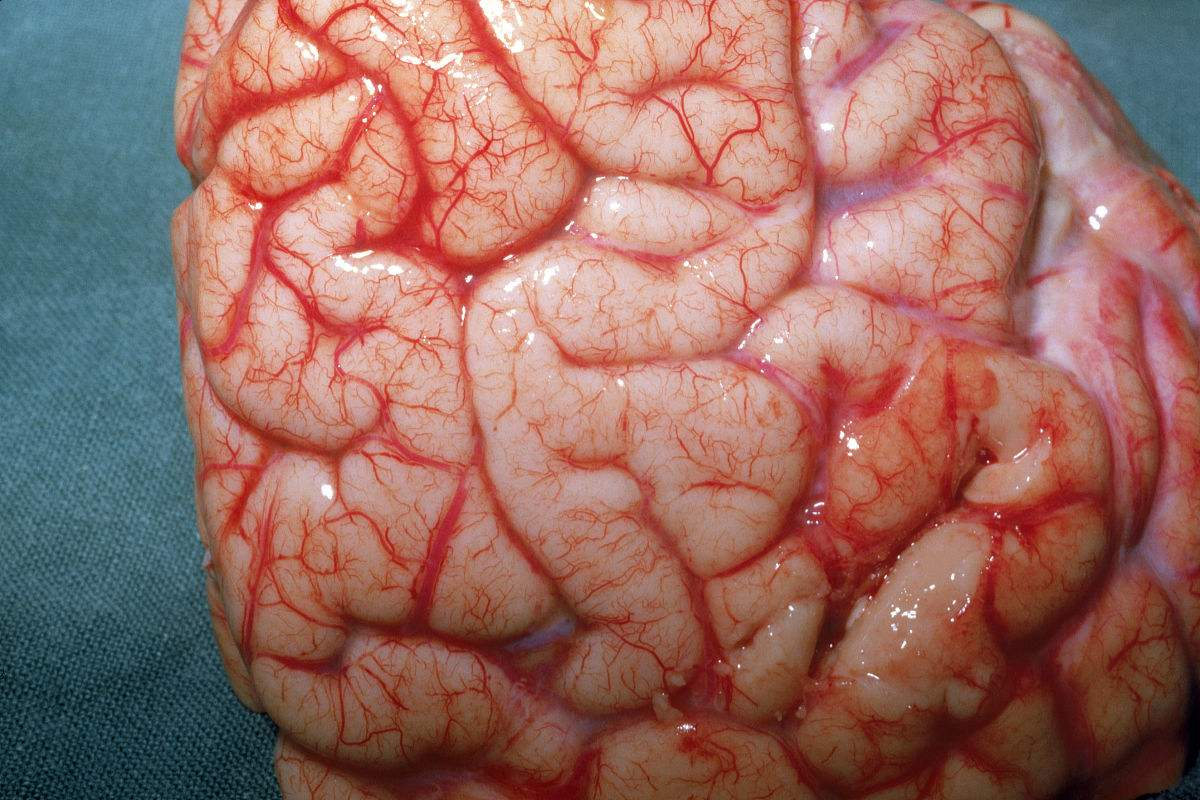
\includegraphics[width=10cm]{Figures/大脑皮层解剖图.jpg}
  \caption{大脑皮层解剖图}\label{大脑皮层解剖图}
\end{figure}

这是一个神经网络游戏的网站,很有意思。\url{http://playground.tensorflowjiaocheng.com/#JJML}
%
%\chapter{深度学习实例}
\section{CNN实例}
CNN(Convolutional Neural Network)是深度学习算法在图像处理领域的一个应用。

利用卷积神经网络将一幅图像的内容与另一幅图像的风格相结合。

\url{https://github.com/jcjohnson/neural-style}

\bibliographystyle{plain}
\bibliography{Citations}
\end{document}
